\chapter{Implementation}
This chapter describes how the design was implemented in the prototype. Furthermore, it describes how the narration system, dubbed the narration-o-matic, was created.

\section{Oculus and Unity with Virtual Reality}
    OVR, camera setup. Regular Oculus hands, with trigger colliders.
\subsection{Narration-o-matic}
    Super cool, maybe too complex narration-o-matic narration system.
    
    \begin{figure}[H]
        \centering
        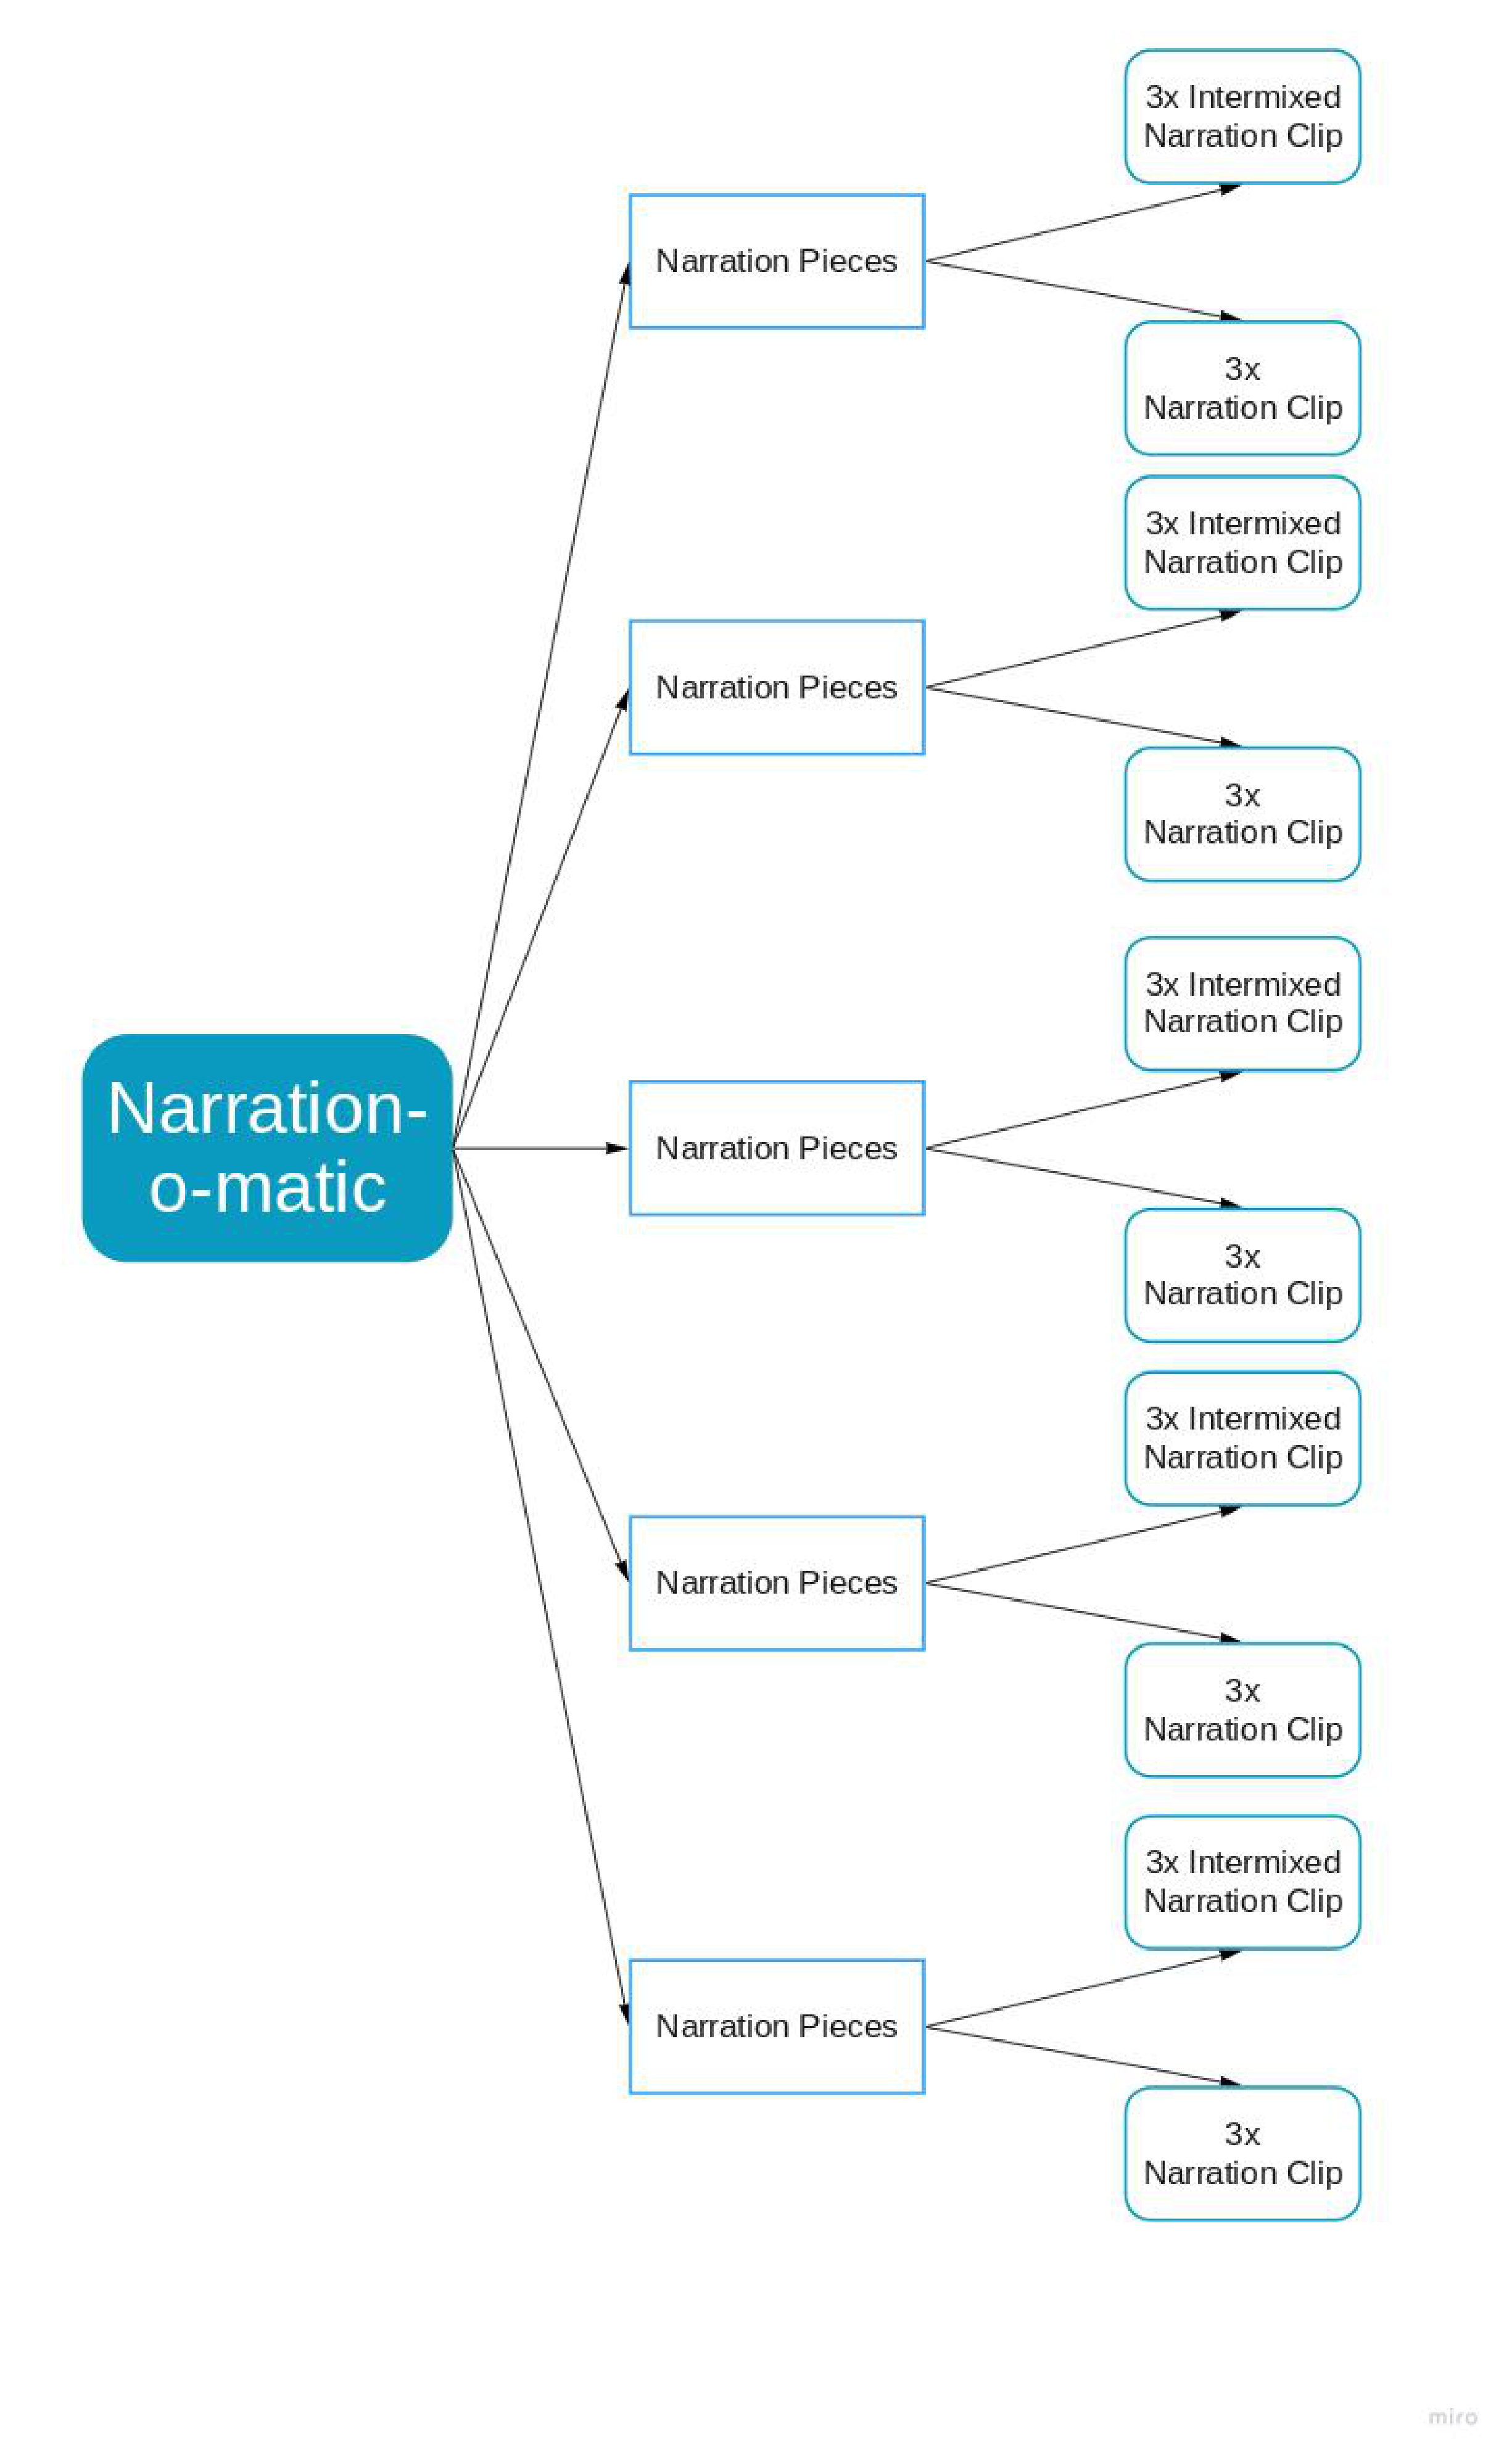
\includegraphics[width=0.6\linewidth]{figure/Implementation/Narration-o-matic-flowchart}
        \caption{The structure of the narration system called the narration-o-matic, showing the different narration pieces, each containing the intermixed, and overloaded clips.}
        \label{fig:narration-o-matic}
    \end{figure}
\subsection{Interactions}
    Grabbing re-parenting transforms, and setting kinematics of grabbed object.

\subsection{Models}
    The car model.

